% !TEX root = ../tex/4-3.tex
% 第4章：本文は青、補足は緑
\newcommand{\asmain}{%
    \setbeamercolor{frametitle}{fg=white,bg=main}%
    \setbeamercolor{structure}{fg=main}%
    \setbeamercolor{itemize item}{fg=main}%
    \setbeamercolor{itemize subitem}{fg=main}%
    \setbeamercolor{enumerate item}{fg=main}%
}
\newcommand{\assuppl}{%
    \setbeamercolor{frametitle}{fg=white,bg=examplecol}%
    \setbeamercolor{structure}{fg=examplecol}%
    \setbeamercolor{itemize item}{fg=examplecol}%
    \setbeamercolor{itemize subitem}{fg=examplecol}%
    \setbeamercolor{enumerate item}{fg=examplecol}%
}
% フレームタイトルの「補足」だけを□で囲む
\newcommand{\supplmark}{%
    \setlength{\fboxsep}{1.5pt}%
    \setlength{\fboxrule}{0.7pt}%
    \fbox{\textbf{補足}}%
}
\asmain


%=============================================
\begin{frame}{4.2から4.3へ}
    \begin{block}{ここまで}
        前向きSDEと逆時間SDE・PF-ODEで、\\
        連続時間のスコア拡散の枠組みを見た。
    \end{block}
    \begin{block}{ここから（スライド4.3＝論文4.4）}
        ドリフト$\bm{f}$と拡散$g$の具体例を入れる。\\
        \textbf{VE SDE}（NCSN）と\textbf{VP SDE}（DDPM）を対応づける。
    \end{block}
\end{frame}
%=============================================
\asmain
\begin{frame}{4.3 の位置づけ}
    \begin{block}{この節の役割}
        一般のScore SDEを、よく使う二つのスケジュールに落とす
    \end{block}
    \begin{enumerate}
        \item \textbf{表4.1}\\
        VE / VPのドリフト・拡散・核・事前分布を一覧する
        \item \textbf{VE SDE}\\
        ドリフトなし＋分散が増える過程 $\;\leftrightarrow\;$ NCSN
        \item \textbf{VP SDE}\\
        線形収縮＋分散が保たれる過程 $\;\leftrightarrow\;$ DDPM
        \item \textbf{（補足）核の導出}\\
        線形SDEの平均・分散ODEから$p_t(\bm{x}_t|\bm{x}_0)$を得る
    \end{enumerate}
\end{frame}
%=============================================
\section{表4.1：VEとVP}
\asmain
\begin{frame}{区切り：表4.1 VE / VP}
    \tableofcontents[currentsection]
\end{frame}
%=============================================
\asmain
\begin{frame}{表4.1：前向きSDEのまとめ}
    \centering
    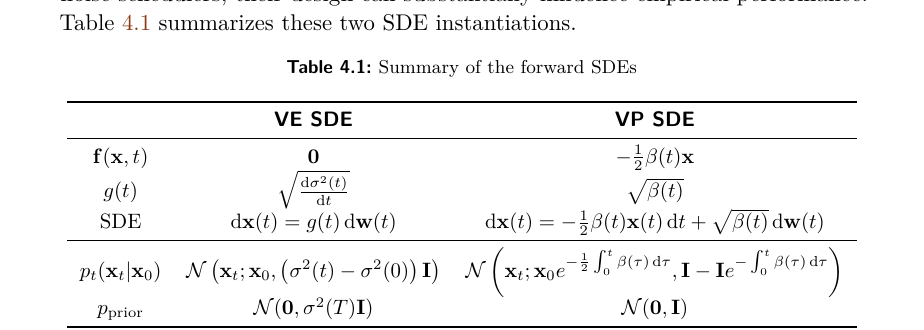
\includegraphics[width=\textwidth,height=0.72\textheight,keepaspectratio]{table-4-1.png}
\end{frame}
%=============================================
\asmain
\begin{frame}{読み方：何が違うか}
    \begin{columns}[T,onlytextwidth]
        \begin{column}{0.48\textwidth}
            \begin{block}{VE}
                $\bm{f}=\bm{0}$。\\
                ノイズだけを足して分散を増やす。\\
                事前は$\mathcal{N}(\bm{0},\sigma^{2}(T)\bm{I})$。
            \end{block}
        \end{column}
        \begin{column}{0.48\textwidth}
            \begin{block}{VP}
                $\bm{f}=-\tfrac12\beta(t)\bm{x}$。\\
                原点へ引きつつ拡散する。\\
                事前は$\mathcal{N}(\bm{0},\bm{I})$。
            \end{block}
        \end{column}
    \end{columns}
    \vfill
    どちらも条件付きはガウスで閉じ、スコアが陽に書ける。\\
    スケジューラの選び方は実験性能に効く。
\end{frame}
%=============================================
\section{VE SDE}
\asmain
\begin{frame}{区切り：VE SDE}
    \tableofcontents[currentsection]
\end{frame}
%=============================================
\asmain
\begin{frame}{VE SDEの定義}
    \begin{block}{成分}
        \begin{itemize}
            \item ドリフト：$\bm{f}=\bm{0}$
            \item 拡散：$g(t)=\sqrt{\dfrac{d\sigma^{2}(t)}{dt}}$（$\sigma(t)$は設計する）
        \end{itemize}
    \end{block}
    前向きSDE：
    \[
        d\bm{x}(t)
        =
        \sqrt{\dfrac{d\sigma^{2}(t)}{dt}}\,
        d\bm{w}(t)
        \tag{4.4.1}
    \]
\end{frame}
%=============================================
\asmain
\begin{frame}{VEの摂動核と事前}
    \begin{block}{摂動核}
        \[
            p_t(\bm{x}_t\mid\bm{x}_0)
            =
            \mathcal{N}\!\bigl(
                \bm{x}_t;\,
                \bm{x}_0,\,
                \bigl(\sigma^{2}(t)-\sigma^{2}(0)\bigr)\bm{I}
            \bigr)
        \]
    \end{block}
    \begin{block}{事前}
        $\sigma(t)$が増加で$\sigma^{2}(T)\gg\sigma^{2}(0)$なら
        \[
            p_{\mathrm{prior}}
            :=
            \mathcal{N}(\bm{0},\sigma^{2}(T)\bm{I})
        \]
    \end{block}
\end{frame}
%=============================================
\asmain
\begin{frame}{VE $\leftrightarrow$ NCSN}
    典型的なスケジュール（$t\in(0,1]$）：
    \[
        \sigma(t)
        :=
        \sigma_{\min}
        \left(\dfrac{\sigma_{\max}}{\sigma_{\min}}\right)^{t}
    \]
    分散列は幾何数列になる。
    \begin{block}{対応}
        NCSNは、このVE SDEを時間離散化したものである（4.1.1）。\\
        $\bm{x}_t=\bm{x}_0+\text{（増えた分散）}^{1/2}\bm{\epsilon}$の形が、\\
        第3章の$\bm{x}+\sigma\bm{\epsilon}$と同じ族である。
    \end{block}
\end{frame}
%=============================================
\section{VP SDE}
\asmain
\begin{frame}{区切り：VP SDE}
    \tableofcontents[currentsection]
\end{frame}
%=============================================
\asmain
\begin{frame}{VP SDEの定義}
    $\beta:[0,T]\to\mathbb{R}_{\ge 0}$をノイズスケジュールとする。
    \begin{block}{成分}
        \begin{itemize}
            \item ドリフト：$\bm{f}(\bm{x},t)=-\tfrac12\beta(t)\bm{x}$
            \item 拡散：$g(t)=\sqrt{\beta(t)}$
        \end{itemize}
    \end{block}
    前向きSDE：
    \[
        d\bm{x}(t)
        =
        -\tfrac12\beta(t)\bm{x}(t)\,dt
        +
        \sqrt{\beta(t)}\,d\bm{w}(t)
        \tag{4.4.2}
    \]
\end{frame}
%=============================================
\asmain
\begin{frame}{VPの摂動核と事前}
    \begin{block}{摂動核}
        \[
            \resizebox{0.95\textwidth}{!}{$
            p_t(\bm{x}_t\mid\bm{x}_0)
            =
            \mathcal{N}\!\Bigl(
                \bm{x}_t;\,
                \bm{x}_0\,e^{-\frac12\int_0^t\beta(\tau)\,d\tau},\,
                \bigl(1-e^{-\int_0^t\beta(\tau)\,d\tau}\bigr)\bm{I}
            \Bigr)
            $}
        \]
    \end{block}
    \begin{block}{事前}
        \[
            p_{\mathrm{prior}}:=\mathcal{N}(\bm{0},\bm{I})
        \]
    \end{block}
    平均・共分散が既知のガウスなので、スコアも閉じた形で書ける。
\end{frame}
%=============================================
\asmain
\begin{frame}{VP $\leftrightarrow$ DDPM}
    典型スケジュール（$t\in[0,1]$）：
    \[
        \beta(t)
        :=
        \beta_{\min}+t(\beta_{\max}-\beta_{\min})
    \]
    \begin{block}{対応}
        DDPMは、このVP SDEの時間離散化である（4.1.1）。\\
        信号は$e^{-\frac12\int\beta}$で縮み、分散は$1-e^{-\int\beta}$へ近づく。\\
        これが第2章の$\bar\alpha_t$型の連続時間版である。
    \end{block}
\end{frame}
%=============================================
\section{（補足）摂動核の導出}
\assuppl
\begin{frame}{区切り：\supplmark\;摂動核の導出}
    \tableofcontents[currentsection]
\end{frame}
%=============================================
\assuppl
\begin{frame}{\supplmark：線形SDEなら核はガウス}
    ドリフトが$\bm{f}(\bm{x},t)=f(t)\bm{x}$のとき、前向きは線形SDE：
    \[
        d\bm{x}(t)=f(t)\bm{x}(t)\,dt+g(t)\,d\bm{w}(t)
    \]
    $p_{\mathrm{data}}$が非ガウスでも、条件付き過程$\bm{x}_t\mid\bm{x}_0$はガウスのまま。
    \[
        p_t(\bm{x}_t\mid\bm{x}_0)
        =
        \mathcal{N}\bigl(\bm{x}_t;\,\bm{m}(t),\,P(t)\bm{I}\bigr)
    \]
    \begin{exampleblock}{ねらい}
        平均$\bm{m}$とスカラー分散$P$のODEを解けば、核が閉じる。
    \end{exampleblock}
\end{frame}
%=============================================
\assuppl
\begin{frame}{\supplmark：平均・分散のODE}
    \[
        \dfrac{d\bm{m}}{dt}=f(t)\bm{m},
        \qquad
        \dfrac{dP}{dt}=2f(t)P+g^{2}(t)
        \tag{4.4.3}
    \]
    積分因子$E(s\to t)=\exp\bigl(\int_s^t f(u)\,du\bigr)$を使うと
    \[
        \bm{m}(t)=E(0\to t)\,\bm{x}_0,
        \qquad
        P(t)=\int_0^t E^{2}(s\to t)\,g(s)^{2}\,ds
        \tag{4.4.4}
    \]
    （初期は$\bm{m}(0)=\bm{x}_0$、$P(0)=0$）。
\end{frame}
%=============================================
\assuppl
\begin{frame}{\supplmark：例 VE}
    $f\equiv 0$、$g(t)=\sqrt{d\sigma^{2}/dt}$のとき
    \[
        \dfrac{d\bm{m}}{dt}=\bm{0}
        \;\Rightarrow\;
        \bm{m}(t)=\bm{x}_0
    \]
    \[
        \dfrac{dP}{dt}=\dfrac{d\sigma^{2}}{dt}
        \;\Rightarrow\;
        P(t)=\sigma^{2}(t)-\sigma^{2}(0)
    \]
    よって
    \[
        p_t(\bm{x}_t\mid\bm{x}_0)
        =
        \mathcal{N}\!\bigl(
            \bm{x}_t;\,\bm{x}_0,\,
            \bigl(\sigma^{2}(t)-\sigma^{2}(0)\bigr)\bm{I}
        \bigr)
    \]
\end{frame}
%=============================================
\assuppl
\begin{frame}{\supplmark：例 VP}
    $f(t)=-\tfrac12\beta(t)$、$g(t)=\sqrt{\beta(t)}$、$B(t)=\int_0^t\beta$。
    \[
        \bm{m}(t)=e^{-\frac12 B(t)}\bm{x}_0,
        \qquad
        P(t)=1-e^{-B(t)}
    \]
    よって
    \[
        p_t(\bm{x}_t\mid\bm{x}_0)
        =
        \mathcal{N}\!\bigl(
            \bm{x}_t;\,
            e^{-\frac12 B(t)}\bm{x}_0,\,
            \bigl(1-e^{-B(t)}\bigr)\bm{I}
        \bigr)
    \]
    \begin{exampleblock}{要点}
        表4.1の核は、このODEの閉じた解である。
    \end{exampleblock}
\end{frame}
%=============================================
\asmain
\begin{frame}{4.3 全体のまとめ}
    \begin{enumerate}
        \item \textbf{VE}：ドリフトなし、分散増加。NCSNの連続時間版。
        \item \textbf{VP}：線形収縮＋$\sqrt{\beta}$拡散。DDPMの連続時間版。
        \item どちらも線形ガウスなので$p_t(\bm{x}_t\mid\bm{x}_0)$が閉じる。
        \item （補足）核は平均・分散ODE（4.4.3）（4.4.4）から来る。
    \end{enumerate}
    \begin{block}{次へ}
        スライド4.4では、核$p_t(\bm{x}_t\mid\bm{x}_0)$を先に置く見方を整理する。
    \end{block}
\end{frame}
%=============================================
\asmain
\begin{frame}{4.3 全体のまとめ：一本の流れ}
    \begin{block}{今日の道筋}
        一般SDE
        $\;\to\;$
        VE（NCSN）/ VP（DDPM）
        $\;\to\;$
        閉じた摂動核
        $\;\to\;$
        （補足）モーメントODE
    \end{block}
    \begin{block}{核心}
        「どの$\bm{f},g$か」を決めると、信号の残り方とノイズの増え方が決まり、\\
        学習で使う条件付き分布が具体化する。
    \end{block}
\end{frame}
